\documentclass[a4paper,10pt]{article}
\usepackage[utf8]{inputenc}

\usepackage{blindtext}
\usepackage{enumitem}
\usepackage{xcolor}

\usepackage{amsmath}
%\usepackage[bottom]{footmisc}
\usepackage{setspace}
\usepackage[font=small]{caption}
\usepackage{pdfpages}
\usepackage{natbib} 
\usepackage{graphicx}
%\usepackage{wrapfig}
\usepackage{lscape}
\usepackage{rotating}
\usepackage{epstopdf}
\usepackage{caption}
%\usepackage{blindtext}
\usepackage{fancyhdr}

\bibliographystyle{abbrv}

%\bibliographystyle{ieeetr}

%opening
\title{PRDM9 zinc finger array evolution}
\author{Diego A. Hartasánchez, Laurent Duret, Nicolas Lartillot}

\begin{document}

\maketitle

\begin{abstract}

\end{abstract}


\section{Introduction}


\begin{itemize}

 \item Meiotic recombination occurs preferentially in delimited regions of the genome known as recombination ``hotspots'' in many species. In humans, mice, cattle and possibly many other vertebrate species \cite{Baker2017} the location of recombination hotspots is determined by the binding of the PR domain containing 9 protein (PRDM9) (cite Myers and others). 
 
 \item Double-strand break biased gene conversion leads to erosion of PRDM9 binding motifs and hence, to the ``hotspot paradox'' which, in the present context would state the following: if PRDM9 binding determines the location of DSBs, how is it that recombination concentrates in hotspots if by the same recombination mechanism PRDM9 binding motifs are expected to erode and ultimately disappear? 
 \item Ubeda and Wilkins \cite{Ubeda2011} and Latrille \textit{et al.} \cite{Latrille2017} investigated a possible solution to the ``hotspot paradox'' by modeling Red-Queen dynamics on PRDM9 evolution, whereupon new PRDM9 alleles would be favorably selected since old alleles would have eroded their binding targets.
 \item PRDM9 consistently shows elevated $dN/dS$ ratios \cite{Oliver2009, Thomas2009, Groeneveld2012, Schwartz2014} at the three zinc-finger residues that enter in contact with DNA upon binding \cite{Wolfe2000b}, suggesting that non-synonymous mutations at these positions might be a consequence of evolutionary pressure on PRDM9, in particular, positive selection for new PRDM9 alleles that recognize new motifs that have not been eroded. 
 \item Resolution of the model demands a high mutation rate since selection is not diversifying. That is, increasing positive selection on PRDM9 alleles with non-eroded targets does not increase PRDM9 diversity. Rather, observed levels of diversity can only be achieved by having an elevated raw mutation rates. 
 \item Indeed, high mutation rate has been observed in PRDM9. For example, the zinc finger array length has a mutation rate (copy-number change rate) of 1e-5 \cite{Jeffreys2013}. Since PRDM9's zinc finger array is responsible for DNA binding, it seems plausible that the high mutation rate in PRDM9 is most likely due to its minisatellite-like structure. 
 \item Recurrence of the same zinc finger at different positions in the array and lack of synonymous differences between them \cite{Oliver2009, Thomas2009} might be generated by unequal crossing over and/or gene conversion within the array \cite{Grey2018}. The concerted evolution of zinc fingers within PRDM9 is a phenomenon that has not been explicitly modeled. 
 \item Specific modeling of PRDM9 zinc finger array structure allows us to envisage possible mechanisms through which the observed PRDM9 mutation rate can be attained. 
 \item Explicit inclusion of the PRDM9 zinc finger structure into the model introduces potentially important differences with respect to Latrille et al.'s infinite sites model \cite{Latrille2017}. Scaling behaviour might be altered. 
\end{itemize}


\section{Methods}

\subsection{Model}
Our model is based on Latrille et al.'s \cite{Latrille2017} model. Differences between models are regarding the explicit simulation of internal structure within each PRDM9 allele and the mutational processes involved (see \ref{Novelties}). The backbone of the model, however, remains the same:
\begin{itemize}
 \item We model a Wright-Fisher population of size $N_e$ with mutation and selection. Each individual is represented by two PRDM9 alleles belonging to their corresponding allelic classes. PRDM9 binding sites are note explicitly modeled. Each allelic class $i$ has a completely different set of targets and each set is initially equally commmon in the genome. 
 \item We will denote as $x_{i,t}$ the frequency of allelic class $i$ at time $t$, and $K_t$ the total number of PRDM9 allelic classes segregating in the population at time $t$.
 \item Every generation, the PRDM9 locus mutates with a certain probability $\mu$. Details regarding the mutation process are given in section \ref{Novelties}.
 \item Every generation, PRDM9 motifs are eroded by dBGC, and as they are eroded, PRDM9 allelic classes recognizing such motifs will decrease in activity. Each allelic class $i$ will have a \textit{recombination activity}, $\theta_i$. A diploid individual, with PRDM9 alleles belonging to allelic classes $i$ and $j$ will have a recombination activity of 
 \begin{equation}
  R_{ij} = \dfrac{\theta_{i,t} + \theta_{j,t}}{2}
 \end{equation}
 \item The recombination activity of allelic class $i$ will decrease proportionally to its frequency in the population since gene conversion events (happening at rate $g$ per DSB) at allelic class' $i$ binding sites occurs at a rate proportional to the number of DSBs initiated at those sites. A gene conversion will only affect the binding site if it has an inactivating mutation, which occurs at rate $v$. The substitution rate of inactiviating mutations at allelic class' $i$ binding sites will be the mutation rate at population level, $2 N_{e}v$, multiplied by its fixation probability, $2 g x_{i,t}$. The change in recombination activity of allelic class $i$ will then be:
 \begin{equation}
  \dfrac{\mathrm{d} \theta_{i,t}}{\mathrm{d}t} = - 2 N_e v 2 g x_{i,t} \theta_{i,t} = - \rho x_{i,t} \theta_{i,t},
 \end{equation}
 where $\rho = 4 N_e vg$ is the population-scaled erosion rate.
\item Every generation, PRDM9 individuals are selected according to their fitness, which is a function of their relative recombination activity. In particular, we consider the fitness function to be a power-law function
\begin{equation}
 f(R)=R^\alpha,
\end{equation}
such that the fitness of an individual with allelic classes $i$ and $j$ will be:
\begin{equation}
 f_{ij}=\bigg(\dfrac{\theta_{i,t} + \theta_{j,t}}{2}\bigg)^\alpha,
\end{equation}
where $\alpha$ is a parameter of our model. Basically, selection against PRDM9 alleles with lower recombination activity is stronger for larger values of $\alpha$.
\item $w_{i,t}$ is the fitness induced by allelic class $i$ at time $t$, which is calculated by averaging it out across all heterozygous backgrounds, such that
\begin{equation}
 w_{i,t} = w(\theta_{i,t})=\sum_{j=1}^{K_t}{x_{j,t}f_{ij}}=\sum_{j=1}^{K_t}{x_{j,t}\bigg(\dfrac{\theta_{i,t}+\theta_{j,t}}{2}\bigg)^\alpha}.
\end{equation}
and the mean population fitness being
\begin{equation}
 \bar{w} = \sum_{i=1}^{K_t}{x_{i,t}w_{i,t}}.
\end{equation}
\item Hence, at any time $t$ we can calculate the selection coefficient, $s_0$, associated with a new arising allelic class (with activity equal to 1) by calculating its fitness contribution compared to the mean population fitness:
\begin{equation}
 s_0 = \dfrac{w(1) - \bar{w}}{\bar{w}}.
\end{equation}
\item For further details of the model please refer to Latrille et al. \cite{Latrille2017}.

\subsection{Novelties of the model}
\label{Novelties}
\item We have explicitly modeled part of the internal structure of PRDM9, in particular, its zinc finger array. Each PRDM9 allele is represented as a sequence of $N_{finger}$ zinc fingers ($N_{finger} = 10$, if not stated otherwise). Each zinc finger is represented by three aminoacids, that represent the positions -1, 3, and 6 of each zinc finger which correspond to the aminoacid residues that come in contact with DNA upon PRDM9 binding \cite{Wolfe2000b}. There are $A$ possible aminoacids that can occupy each of the three positions at any zinc finger. Therefore, the total number of possible zinc fingers is $A^3$. We will consider two PRDM9 alleles to be different if there is any difference between them at any of the $3N_{finger}$ residues. %In other words, two alleles will be the same if they share the same aminoacid sequence.
\item Even though all zinc fingers of the array bind to DNA, in humans and mice, only a subset of zinc fingers determine its DNA binding motif. In the case, for example, of the major PRDM9 allele in human European populations, the up to last 5 zinc fingers in the array were predicted to bind to a 13-bp slightly degenerate motif (cite Myers and other papers). Accordingly, in our model, only the first $N_{bind}$ fingers of the array ($N_{bind} = 3$, if not stated otherwise), which we will refer to as the \textit{relevant} zinc fingers, will determine the binding site of each PRDM9 allele. We will assume that any aminoacid difference at any of the first $3N_{bind}$ positions will imply a recognition of a different binding motif. Therefore, any two alleles with identical zinc fingers at the relevant positions will be considered to belong to the same \textit{allelic class}, since they will recognize the same binding motif. Note that in Latrille et al. \cite{Latrille2017} any two alleles represented in fact two different allelic classes. 
 \item Every generation, PRDM9 alleles can suffer a point mutation and/or an gene conversion mutation among two zinc fingers. Point mutations occurs at a per position per generation rate $u$, being $U=4N_e 3 N_{finger} u$ the population-scaled point mutation rate. A point mutation event will modify the aminoacid residue at any of the $3N_{finger}$ positions of the array (silent mutations are allowed). Interfinger gene conversion (IGC) mutations occur at a per zinc finger per generation rate $c$, with $C=4Nc N_{finger}$ being the population-scaled IGC rate. An IGC event will happen between two randomly-chosen zinc fingers in which one will be the donor and the other one, the acceptor (donor and acceptor must be different). The donor zinc finger will remain the same whereas the acceptor zinc finger will be substituted by the donor zinc finger.  
 Note: The term IGC has been used before to refer to \textit{interlocus gene conversion} \cite{Hartasanchez2014} (cite Dumont), that is, gene conversion between different loci, also called non-allelic or ectopic gene conversion. Since interfinger gene conversion is in itself a form of interlocus gene conversion, we will here use the term IGC to refer to the former without loss of generality. 
 \item We will consider point mutations and IGC mutations to be \textit{effective} only if they modify the allelic class of the allele they fall upon. 
 \item An extension of the model includes duplication and delection of zinc fingers.
 %\item INCLUDE DESCRIPTION OF DIVERSITY MEASURES: DEFINE ALLELIC CLASS, ALLELE AND ZINC FINGER DIVERSITY.
\end{itemize}


 %\subsection{Novelties of the model}
 
% Interfinger gene conversion: DESCRIBE the homogenizing effects and diversifying effects here, without explicit connection with allelic class or zinc finger diversity. 
  
 Explicit simulation of the zinc finger structure of PRDM9 alleles allows us to explore PRDM9 evolution from a different perspective, namely, from the evolution of zinc fingers themselves. Previous theoretical and simulation studies \cite{Latrille2017, Ubeda2019} have ignored the mutation landscape and internal structure of PRDM9.
 %as allelic classes, since each allelic class recognizes a different binding motif, wheareas we retain the term ``alleles'' to refer to unique aminoacid sequenceS. Two alleles may belong to the same allelic class if they recognize the same binding motif. 
 By focusing on PRDM9's zinc finger array structure we have tested, for the first time to our knowledge, the hypothesis that the minisatellite-like structure of PRDM9 evolving under Red-Queen dynamics might explain the high mutation and turnover rate of this protein, which could in turn contribute to the resolution of the hotspot paradox. 
 
We focus, in particular, on the effect that IGC has on zinc finger diversity within the array and how that diversity is translated into allelic class diversity. Theoretical and simulation studies of IGC \cite{Innan2003, Hartasanchez2014} have shown that IGC can have two distinct consequences on diversity. On the one hand, high IGC rates have a homogenizing effect, which lowers diversity between regions. On the other hand, IGC at low rates increases within-region diversity by exchanging variants between regions. In the particular context of PRDM9, this implies interesting effects on zinc finger and allelic class diversity. 
  
 %Striedner 2017, Yo escribo: Binding affinity of PRDM9 is certainly more complex than the reduction of PRDM9 binding to three out of ten zinc fingers is a simplified version of reality. 
  %Neale 2010... resumen de los resultados recientes de prdm9... propone possible rapid evolution due to recombination slippage en prdm9.
  %Capilla 2016 Resumen de mammalian recombination. Buenas imágenes y resumen de prdm9
  %Buard2014 Diversity of prdm9 in mice... possibility to count allelicClasses Alleles and zinc fingers
  %\item Non-allelic homologous recombination can ocurr between zinc fingers along the array generating alleles of different lengths. 


\section{Scaling behaviour}



Observing the scaling behaviour of the model under its parameters is essential in order to understand the forces underlying changes in measurable quantities such as the mean recombination activity of segregating alleles, diversity and selection coefficient. We have carried out long simulations exploring a range of each parameter while keeping all other parameters constant (see Figures \ref{RecAct_scaling}, \ref{ACdiv_scaling}, and \ref{ZnfDiv_scaling}).



\subsection{Mean recombination activity}
The mean recombination activity is the frequency-weighted average of the recombination activity of all segregating allelic classes averaged across the entire simulation. 
 \begin{equation}
 R =  \langle R_t \rangle = \bigg \langle \sum_{i \epsilon K_t} x_{i,t} \theta_{i,t} \bigg \rangle.
\end{equation}
Dependence of $R$ on parameters $\alpha$, $\rho$ and $U$ are as expected and in accordance with the scaling behaviour shown by Latrille et al. \cite{Latrille2017}. Higher values of $\alpha$ imply a higher average recombination activity (Figure \ref{RecAct_scaling}A) and a faster turnover rate since, all else being equal, new alleles will invade the population with a higher frequency under a stonger selective regime. Accordingly, a higher point mutation rate implies a faster generation of new alleles and, hence a faster turnover rate and lower erosion (Figure \ref{RecAct_scaling}C). Correspondingly, higher $\rho$ values render lower values of $R$ since segregating alleles erode their targets at a faster rate (Figure \ref{RecAct_scaling}B). However, interfinger gene conversion rate, $C$, has a non-monotonous effect on $R$. Increasing $C$ increases $R$ values up to a certain point (around $C = 1$), in a behaviour that is equivalent to that observerd with an increase in point mutation rate. Nevertheless, for values above ($C = 1$), an increase in $C$ causes a decrease in $R$. \textit{A priori}, there are many possible causes for this observation. In any case, observing the effect of $C$ variation on other summary statistics such as allelic class diversity, $D_{AC}$, and zinc finger diversity, $D_{ZF}$ can provide a possible explanation. 


\subsection{Allelic class diversity}
DEFINITION OF AC DIV
One of the main findings of Latrille et al. \cite{Latrille2017} was that in their model, in order to achieve high diversity, high mutation rates needed to be invoked. In other words, increasing selective pressure did not cause an increase in diversity. Surprisingly, with the inclusion of interfinger gene conversion we observe a completely different behaviour. As can be observed in Figure \ref{ACdiv_scaling}A, higher values of $\alpha$ increase $D_{AC}$. The same is the case of $\rho$. Although the simulations in Latrille et al. \cite{Latrille2017} already showed a slight increase in diversity for higher erosion rates, the effect under our model is considerably stronger, observing a two-fold increase in $D_{AC}$ with a 4-orders-of-magnitude increase in $\rho$ (Figure \ref{ACdiv_scaling}B).

As expected, an increase in point mutation rate, $U$, increases $D_{AC}$ (Figure \ref{ACdiv_scaling}C). This behaviour is identical to that observed by Latrille et al. \cite{Latrille2017}. However, increasing interfinger gene conversion rate, $C$, has a non-monotonous effect on $D_{AC}$ (Figure \ref{ACdiv_scaling}D). For values of $C < 10$, $D_{AC}$ increases with increasing $C$, suggesting a behaviour akin to increasing $U$, while for values of $C > 10$, $D_{AC}$ decreases with increasing $C$ implying a negative returns relation between $C$ and $D_{AC}$ above a certain $C$ threshold. 

To understand this non-monotonous effect of interfinger gene conversion on allelic class diversity we can step back and explore the effect of $C$ variation on zinc finger diversity, $D_{ZF}$, which is more straightforward, and then analyse how zinc finger diversity translates into allelic class diversity. 


\subsection{Zinc finger diversity}
DEFINITION OF ZF DIV
Zinc finger diversity, $D_{ZF}$, dependence on $\alpha$ and $\rho$ shows a clear difference between presence and absence of IGC. In the absence of IGC, $D_{ZF}$ does not depend on $\alpha$ or $\rho$. In the presence of IGC, $D_{ZF}$ increases slightly with increasing values of $\alpha$ (Figure \ref{AC_ZF_div_scaling}E) and increasing values of $\rho$ (Figure \ref{AC_ZF_div_scaling}F). Furthermore, the presence of IGC reduces $D_{ZF}$ to a large extent despite an increase in total number of potential mutational events and reduces the variance in $D_{ZF}$. This can only be understood when observing the effect that the IGC rate $C$ has on $D_{ZF}$ (Figure \ref{AC_ZF_div_scaling}H). As explained in \ref{Novelties}, interfinger gene conversion causes an homogeneization of zinc fingers, decreasing their overall diversity. Increasing $C$ decreases $D_{ZF}$ (Figure \ref{AC_ZF_div_scaling}H) in clear contrast with the effect of increasing the point mutation rate, $U$, which increases $D_{ZF}$ (Figure \ref{AC_ZF_div_scaling}G). 

How come then, does allelic class diversity increase with the presence of IGC and with increasing IGC rate (up to a certain threshold) despite zinc finger diversity decreasing monotonously with increasing IGC rate? The answer lies in the combinatorial force induced by IGC.


\section{Interfinger gene conversion effects on diversity}

Our model provides an interesting setup:
\begin{itemize}
 \item Point mutations can generate novel zinc fingers at any position in the array, generating, in turn, a new PRDM9 allele. 
 \item However, this new allele will only give rise to a new allelic class if the new zinc finger is born within relevant zinc fingers of the array or once it is \textit{transferred} via IGC to the relevant zinc fingers.
 \item Since selection only acts upon allelic classes, for a new allele (or a new zinc finger) to rise in frequency it must be within the relevant positions of the array, or occasionaly, it could rise in frequencY if it were at high linkage disequilibrium with another zinc finger within the relevant positions.
 \item After a new zinc finger is born, it can potentially give rise to multiple new allelic classes by generating different permutations of segregating zinc figers at the relevant positions in the array. The number of new allelic classes generated by a specific zinc finger will depend essentially on three factors: on the number of segregating zinc fingers, on the possibility for these zinc fingers to move to other positions in the array (via IGC), on the number of combinations generated (also via IGC), and on the selection pressure favoring new allelic classes.%, among other factors (see Section \ref{section_Quasispecies}).
 %\item Therefore, when measuring diversity we can focus on three different layers of diversity: allelic class, allele or zinc finger diversity. Their interplay is essential to the understanding of PRMD9 evolution.  
 \end{itemize}

 So, there is a mechanistic basis centered around IGC behind the connection between zinc finger and allelic class diversity. On the one hand, IGC reduces zinc finger diversity which will in turn reduce allelic class diversity. On the other hand, IGC allows zinc fingers at non relevant positions to ``jump'' to a relevant position and it also permits the generation of different combinations of segregating zinc fingers within relevant positions, both of which potentially increase allelic class diversity. These two oposing forces are precisely the ones responsible for the non-homogeneus effect of $C$ on $D_{AC}$ (Figure \ref{AC_ZF_div_scaling}D). For values below $C = 20$ the combinatorial force of IGC outcompetes its homogenizing force, which takes over for $C > 20$ values. No matter how powerful IGC's combinatorial power is, if there is no diversity present in the first place, there will be nothing to generate combinations with.  
 
 In other words, zinc finger diversity needs to be high enough for IGC to generate new allelic classes. This is achieved by point mutation and IGC. Increasing $C$ rates proves to be efficient in generating more allelic class diversity, however, above a certain threshold, no matter how high the point mutation rate, increasing IGC will wipe out zinc finger diversity by homogeneization rendering IGC's combinatorial power useless. It will still make combiations, but combinations of the same zinc finger will not be real combinations. 
 
Essentially, by introducing IGC into the model we have modified no only the mutational mechanism, but also the mutational landscape and the effectiveness of mutation events. In an infinite alleles model (i.e. Latrille et al. \cite{Latrille2017}) any mutation on PRDM9 generated a completely novel allele with a completely new and non-eroded set of binding sites. In our model, not only are recurrent mutations possible but there exists the possibility for an IGC event to be silent. We will call ``effective mutations'' those mutations that actually modify the allelic class of the allele on which it happened. How the rate of effective mutation varies with IGC rate will provide more insight into the effect of IGC on diversity measures. 

HERE, I MIGHT INCLUDE EITHER THE BLACK BALL FIGURE (ONLY ZINC FINGER AND ALLELIC CLASS DIV) OR THE FIGURE WITH DIFFERENT COLOR LINES. ASK NICOLAS.
 
 
 
\section{Effective mutation rates}
%Let us consider a very simple scenario in which there is no gene conversion between zinc fingers, and that all the mutational input is coming from point mutations. 


Higher interfinger gene conversion rates imply a higher rate of zinc finger homogenization. As such, under a constant point mutation rate and selective pressure, a higher $C$ will imply a smaller ratio of gene conversion events that will actually be a mutation with respect to the total number of gene conversion events (Figure \ref{FigEffMuts}). That is, higher $C$'s will be associated with a higher chance for a gene conversion event to occur between identical zinc fingers, therefore being ``useless''. We observe this phenomenon both for a neutral regime (black simbols in Figure \ref{FigEffMuts}) and under the Red-Queen selective regime. However, the stronger the selective force the higher the proportion of effective gene conversion mutation events. The higher the selection coefficient, the higher the turnover rate, and the higher the chance for individuals carrying new mutations to invade the population, increasing the chance for gene conversion events to be diversifying. In the case of very high mutation rates and low gene conversion rates, differences between neutral and selective regimes is very small. Additionally, lower point mutation rates imply a lower ratio of effective gene conversion mutations. The reason for the latter observation is that higher point mutation generates diversity whereupon gene conversion can act, esentially by transferring ``new'' zinc fingers, generated by point mutations, to the relevant zinc fingers in the array. 

By increasing gene conversion rate, \textit{ceteris paribus}, there is practically no change in the ratio of effective point mutations relative to the total, except for very high gene conversion rate and point mutation rates, in which we do observe a slight decrease. This makes sense since the homogeneization of zinc fingers does not affect the probability for a new point mutation to generate a new allelic class. Higher selective coefficients increase the ratio of effective point mutations. %This effect might be caused by recurrent mutations, which increase for smaller turnover rates (although I'm not completely certain). 
On the contrary, a higher point mutation rate decreases the ratio of effective point mutations. 

\begin{figure}[htb]
\begin{center}
\leavevmode
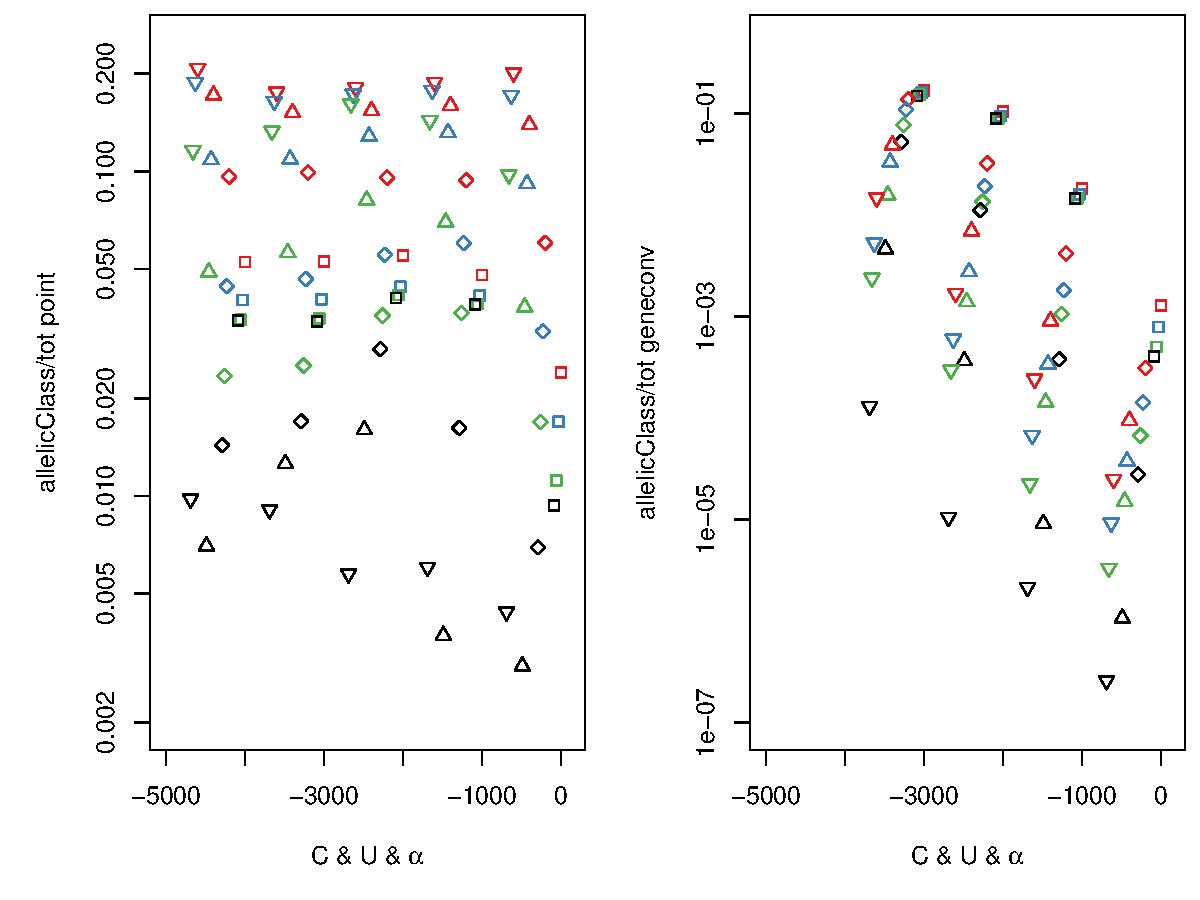
\includegraphics[width=0.95\textwidth] {./Images/Rplot_allelicClassEffVsTot_pointGeneconv.pdf}
\end{center}
\caption{\small{}}
\label{FigEffMuts}
\end{figure}

So, it is clear that there is a link between point mutation and gene conversion that determines the possibility to generate diversifying mutations. A question that we might ask is what is the proportion of new allelic classes generated by point mutation versus those generated by gene conversion mutations. If we ignore the neutral regime, it turns out that the regimes for which the strength of selection (i.e. 4Ns, not to be confused with the selection parameter $\alpha$) is higher are the regimes for which the proportion of new allelic classes generated by gene conversion is highest (see image of gene conversion proportion and 4Ns, red inverted triangles). There are several things of interest regarding these data points: first, the gene conversion effective proportion does not depend on gene conversion rate despite there being four orders of magnitude between different gene conversion rates; second, they correspond to the scenarios of very low point mutation rates; and third, they are the cases for which the efficiency of point mutations is highest (see Figure \ref{FigEffMuts}). 

The fact that both the proportion of effective mutations arising from gene conversion and the fraction of effective point mutations are constant in this scenario of very low mutation rates is in agreement with the mechanism of generation of new allelic classes.
%\begin{enumerate}
% \item A new zinc finger appears in the zinc finger array via point mutation. 
% \item This zinc finger might be born within the binding portion of the array. If it born outside, a gene conversion event might copy this zinc finger to the binding portion of the array.
%  \item Thereafter, gene conversion event can generate many novel allelic classes by copying this zinc finger to other positions within the relevant portion of the array. 
% \item The number of different allelic classes that will contain a particular zinc finger within its binding portion will depend on several parameters and will define the regime in which it is evolving (strong quasi-species vs. weak quasi-species vs. polymorphic vs. sequential).
%\end{enumerate}

%This is a very clear example of the relationship between gene conversion and point mutation rates. In 
For example, in the case of a very low point mutation rate, no matter how high the gene conversion rate, the number of events that will be of use will depend on the availability of segregating zinc fingers, which is dependent on point mutation rate and gene conversion rate. 

For very high gene conversion rates we observe that even the effectivity of point mutations is lower (due mostly to recurrent mutations, most probably). If we look at the proportion of novel allelic classes generated by gene conversion we see that it is extremely low for low gene conversion rates (all new allelic classes are generated by point mutations) and up to 50\% for high gene conversion rates. When comparing this scenario for different values of $\alpha$ we observe that the allelic classes generated by gene conversion are not because of the Red-Queen dynamics since the results for $\alpha=0$ are the same. The only difference between different values of $\alpha$ can be observed for high gene conversion rates. This scenario represents the upper end in point mutation rates, which is up to a point in which gene conversion causes a very small effect. The scenarios in between are the interesting ones, in which there is an interesting equilibrium between gene conversion and point mutation rates. 

THE IMAGE FOR THIS EFFECT IS in page Prop.

ONE THING THAT NEEDS TO BE DISCUSSED IS THE INABILITY TO HAVE AN ADEQUATE MUTATION RATE AS A PARAMETER OF THE MODEL SINCE IT TURNS OUT TO BE DEPENDENT ON THE PARAMETERS OF THE MODEL ITSELF. 

In Latrille et al. \cite{Latrille2017}, the population-scaled mutation rate, $\mu$, was a parameter of the model. Under their infinite alleles model, any mutation of PRDM9 changed its set of binding sites and no recurrent mutations were possible. Analytical aproximations under a weak-erosion regime demonstrated that diversity of PRDM9 scaled with $\mu$ and increasing selection did not increase diversity.

In our model, the mutation-related parameters are the point mutation rate, $U$, and the IGC rate, $C$, but a composed mutation parameter is not a simple function of both. As discussed above, effective mutation rates are dependent on the state of the simulation which depends in a non-homogeneous manner on $C$ and in a complex manner on $C$ and $U$. A direct sequence of the fact that some of the mutation events carried out are not effective in generating allelic classes is that the mutation rate, $\mu$, ceases to be a parameter of the model and becomes, rather, a summary statistic. In that sense we can in fact calculate $\mu$ \textit{a posteriori} by basically counting the number of both point and gene conversion events that modify only the allele or both allele and allelic class of a PRDM9 allele. 





%I really do need to check how many of these point mutations generate a new allelic class but not a novel one. 



 
 
 
 
\section{Selective versus neutral regime}
 
IN THIS SECTION WE COULD TRY TO REACH HIGH LEVEL OF DIVERSITY WITHOUT NEED TO INVOKE VERY HIGH POINT MUTATION RATE BUT A COMBINATION OF POINT MUTATION AND IGC
 

If we observe allelic class, allele and zinc finger diversity as a function of $C$ and $U$ simultaneously we can infer some of the underlying dynamics.
\begin{itemize}
 \item The higher the point mutation rate and the lower the gene conversion rate, the higher the diversity of zinc fingers. Higher point mutation generates new zinc fingers more often, however, gene conversion homogenizes the array, reducing diversity. If we focus on zinc fingers, we can consider point mutation and gene conversion as two opposing forces: point mutation increases diversity, whilst gene conversion reduces diversity. 
 \item This effect, however, is not reflected in the allele diversity. Recall that two alleles are different if they differ in at least one zinc finger at one particular position. We could therefore expect, \textit{a priori}, that higher zinc finger diversity would be translated into allele diversity. This is not the case at all. For gene conversion rates below $C=10$, allele diversity increases with gene conversion rate, contrary to zinc finger diversity. 
 Interestingly, the relation between mutation rates and allele diversity is not linear. For gene conversion rates up to $C=10$, a higher point mutation rate implies more allele diversity. However, when gene conversion rate is very high (i.e. $C=40$ in Figure \ref{AllDiv}) a higher point mutation rate renders a lower allele diversity. 
 PROVIDE EXPLANATION
 \item Allelic class diversity has, to a large extent, the same behaviour as allele diversity although the differences are not as large between different scenarios. 
 %Important... rerun more experiments with high gene conv and low point mut to see if this effect is maintainted. 

 \end{itemize}






 

\begin{figure}[htb]
\begin{center}
\leavevmode
\includegraphics[width=0.95\textwidth] {./Images/scaling_pXCU_RecAct.pdf}
\end{center}
\caption{\small{}}
\label{RecAct_scaling}
\end{figure}

\begin{figure}[htb]
\begin{center}
\leavevmode
\includegraphics[width=0.95\textwidth] {./Images/scaling_pXCU_ACdiv.pdf}
\end{center}
\caption{\small{}}
\label{ACdiv_scaling}
\end{figure}

\begin{figure}[htb]
\begin{center}
\leavevmode
\includegraphics[width=0.95\textwidth] {./Images/scaling_pXCU_ZnfDiv.pdf}
\end{center}
\caption{\small{}}
\label{ZnfDiv_scaling}
\end{figure}


% \begin{figure}[htb]
% \begin{center}
% \leavevmode
% \includegraphics[width=0.95\textwidth] {./Images/scaling_pXCU_4Ns.pdf}
% \end{center}
% \caption{\small{}}
% \label{4Ns_scaling}
% \end{figure}

% \begin{figure}[htb]
% \begin{center}
% \leavevmode
% 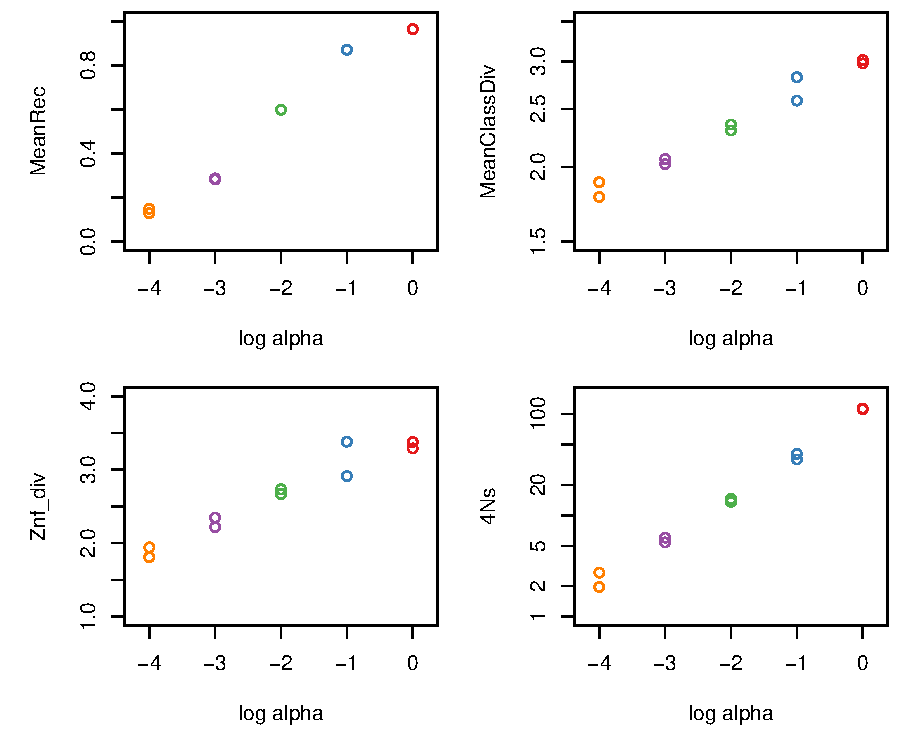
\includegraphics[width=0.95\textwidth] {./Images/scaling_alpha.pdf}
% \end{center}
% \caption{\small{}}
% \label{alphaScaling}
% \end{figure}



\subsection{$\alpha$ scaling}

Higher values of $\alpha$ (i.e. high selection pressure upon new allelic classes) imply a higher average recombination activity (Figure \ref{RecAct_scaling}) and a shorter turnover time  since, all else being equal, new alleles will invade the population with at a higher rate under a stonger selective regime. PRDM9 diversity, on the contrary, is not expected to be affected by changes in $\alpha$, as observed in Latrille et al. \cite{Latrille2017}. However, in our model, allelic class diversity and zinc finger diversity increase with increasing values of $\alpha$ (Figures \ref{ACdiv_scaling} and \ref{ZnfDiv_scaling}). 

\subsection{$\rho$ scaling}

An increase in the erosion rate of PRDM9 binding motif causes, as expected, a decrease in the equilibrium activity (see Figure \ref{RecAct_scaling}). Akin to the effect of variation in $\alpha$ values, we observe an increase in allelic class and zinc finger diversity for higher erosion rates. Although the simulations in Latrille et al. \cite{Latrille2017} already showed a slight increase in diversity for higher erosion rates, the effect under our model is considerably stronger, observing a two-fold increase in allelic class diversity with a 4-orders-of-magnitude increase in $\rho$ (Figure \ref{ACdiv_scaling}). 


\subsection{U scaling}
The effect of increasing the mutation rate is an increase in mean recombination activity (Figure \ref{RecAct_scaling}). The higher the mutation rate, the higher the frequency of appearance of new alleles in the population and the higher the chance for any of these alleles to invade the population. Since invasion of the population by new allelic classes happens more often when mutation rates are higher, the faster the rate and the smaller the erosion of motifs associated to any allelic class. Consequently we also observe an increase in allelic class and zinc finger diversity  (Figures \ref{ACdiv_scaling} and \ref{ZnfDiv_scaling}). Interestingly, for very high point mutation rates, the diversity in zinc fingers is extremely high, but not all of this diversity is ``transferred'' to the zinc fingers relevant in binding specificity, renderring the increase in allelic class diversity higher for higher point mutation rates, but to a much lesser extent than zinc finger diversity (see Section \ref{section_AC_allele_znf_div}).


\subsection{C scaling}
Gene conversion among zinc fingers has effects on summary statistics that make sense once the direct consequences of inter-finger gene conversion are taken into account. Interlocus or ectopic gene conversion is mostly referred to as an homogenizing force in the evolution of gene duplications, for example. However, there is another important effect that is not as well known: when gene conversion rates are low, gene conversion is a diversifying force in the sense that it increases within-locus diversity (\cite{Innan2003, Hartasanchez2014}). Low, but constant rates of gene conversion increase the variation within the duplicated regions.

Under our model, we can observe both of these effects. Firstly, for high gene conversion rates, zinc finger diversity is very low, implying, as expected, that gene conversion homogenizes all zinc fingers. Basically, under high gene conversion rates, shortly after a new point mutation generates a new zinc finger, a gene conversion event will fall upon that zinc finger erasing the new-born zinc finger from the population. Conversely, for low gene conversion rates, zinc finger diversity is high, implying that there is a large number of zinc fingers segregating in the population. 

But how is zinc finger diversity ``translated'' into allelic class diverisity? Within our model, a new allelic class is generated only when a new combination of relevant zinc fingers arises in the population. This can happen through two mechanisms: either a point mutation happens within relevant zinc fingers or a gene conversion event transfers a new zinc finger to the relevant section of the array. So, regarding allelic class diversity, a high gene conversion rate increases the probability to generate a new allelic class. However, this depends in the existing zinc finger diversity. For example, a very high gene conversion rate could, a priori, generate new allelic classes with a higher frequency, however, since a high gene conversion homogenizes the zinc fingers present in the whole of the array, the probability for a gene conversion event to transfer a new zinc finger to the relevant section of the array actually decreases after a certain point. We can observe that the maximum of allelic class diversity is reached for a gene conversion rate of $C=10$. 

EXTEND EXPLANATION


\section{Allelic class, allele and zinc finger diversity}
\label{section_AC_allele_znf_div}
Our model provides an interesting setup:
\begin{itemize}
 \item Point mutations can generate novel zinc fingers at any position in the array, generating, in turn, a new PRDM9 allele. 
 \item However, this new allele will only give rise to a new allelic class if the new zinc finger is born within relevant zinc fingers of the array or once it is ``transferred'' via interfinger gene conversion to the relevant zinc fingers.
 \item Since selection only acts upon allelic classes, for a new allele (or a new zinc finger) to rise in frequency it must be within the relevant positions of the array, or occasionaly, it could rise in frequence if it were at high linkage disequilibrium with another zinc finger within the relevant positions.
 \item After a new zinc finger is born, it can potentially give rise to multiple new allelic classes by generating different permutations of segregating zinc figers at the relvant positions in the array. The number of new allelic classes generated by a specific zinc finger will depend on several factors: on the number of segregating zinc fingers, on the possibility for these zinc fingers to move to other positions in the array (via interfinger gene conversion), on the selection pressure favoring new allelic classes, among other factors (see Section \ref{section_Quasispecies}).
 \item Therefore, when measuring diversity we can focus on three different layers of diversity: allelic class, allele or zinc finger diversity. Their interplay is essential to the understanding of PRMD9 evolution.  
 \end{itemize}


If we observe allelic class, allele and zinc finger diversity as a function of $C$ and $U$ simultaneously we can infer some of the underlying dynamics.
\begin{itemize}
 \item The higher the point mutation rate and the lower the gene conversion rate, the higher the diversity of zinc fingers. Higher point mutation generates new zinc fingers more often, however, gene conversion homogenizes the array, reducing diversity. If we focus on zinc fingers, we can consider point mutation and gene conversion as two opposing forces: point mutation increases diversity, whilst gene conversion reduces diversity. 
 \item This effect, however, is not reflected in the allele diversity. Recall that two alleles are different if they differ in at least one zinc finger at one particular position. We could therefore expect, \textit{a priori}, that higher zinc finger diversity would be translated into allele diversity. This is not the case at all. For gene conversion rates below $C=10$, allele diversity increases with gene conversion rate, contrary to zinc finger diversity. 
 Interestingly, the relation between mutation rates and allele diversity is not linear. For gene conversion rates up to $C=10$, a higher point mutation rate implies more allele diversity. However, when gene conversion rate is very high (i.e. $C=40$ in Figure \ref{AllDiv}) a higher point mutation rate renders a lower allele diversity. 
 PROVIDE EXPLANATION
 \item Allelic class diversity has, to a large extent, the same behaviour as allele diversity although the differences are not as large between different scenarios. 
 %Important... rerun more experiments with high gene conv and low point mut to see if this effect is maintainted. 

 \end{itemize}

 
\begin{figure}[htb]
\begin{center}
\leavevmode
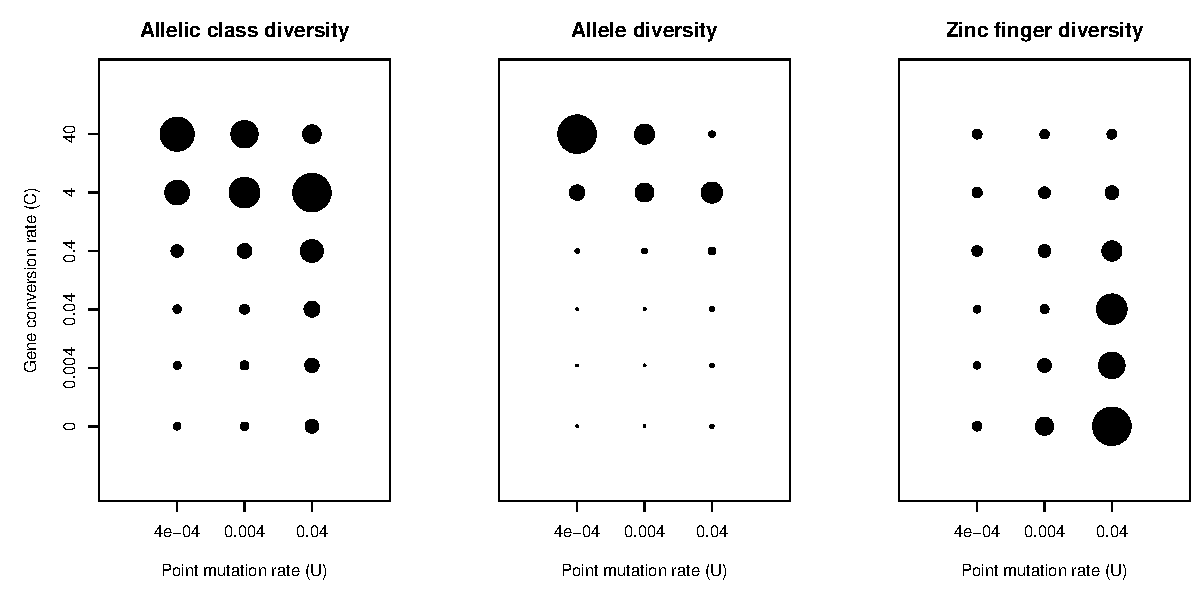
\includegraphics[width=0.95\textwidth] {./Images/prdm9_allRate.pdf}
\end{center}
\caption{\small{}}
\label{AllDiv}
\end{figure}


\section{Quasispecies-like allelic classes}
\label{section_Quasispecies}
For certain parameter regimes, we observe behaviour that can be interpreted as being quasispecies-like. In particular, we observe that several allelic classes appear during a short period of time, erode their binding motifs more or less at the same pace, and dissapear around the same period of time. This phenomenon is observed under high gene conversion rates. Especifically, when existing allelic classes have eroded their binding sites down to a point in which a newly-born allelic class is likely to rise in frequency due to selection, a newly born zinc finger within the binding region in the array is likely to rise in frequency. Under a high gene conversion rate scenario, more allelic classes containing the new zinc finger within the binding region of the array arise shortly after. These new allelic classes will be a subset (or complete set) of all possible combinations of zinc fingers within the binding region of the array that contain at least the new zinc finger in combination with the other zinc fingers that remain at high frequency. This group of newly formed allelic classes containing one zinc finger in particular evolve under a quasispecies-like behaviour which can be defined by the following characteristics:
\begin{itemize}
 \item First, mutations from one allelic class onto the other are frequent (only possible under high gene conversion rates).
 \item Second, their binding motifs decrease in frequency as a group. Even though slight differences in the degree of erosion will arise, these differences will be quickly translated into a raise in frequency of another member of the quasispecies, with the subsequent erosion of the latter's binding motif and a decrease in erosion levels among members of the quasispecies.
 \item Third, dissapearance and reappearance (via gene conversion) of a particular member of the quasispecies is common and bound to erode all members of the quasispecies to more or less the same level. 
 \item Fourth, once the erosion reaches a certain level (this level will mostly depend on parameters $\alpha$ and $\rho$) the cicle starts again with the appearance of a new zinc finger triggering the invasion of the population by a new quasispecies-like allelic class.
\end{itemize}

The number of allelic classes conforming a quasispecies-like group will depend on the number of possible combinations that can be generated with the existing zinc fingers. Under the parameter regimes explored, we only observed quasispecies-like groups of size 7, which is corresponds to the possible combinations of two zinc fingers among three relevant sites minus the already existing allelic class. For example, consider a QACG (quasispecies-like allelic class group) formed by zinc finger A that is replaced by a QACG of zinc finger B. The newly born allelic classes  will have combinations of zinc fingers A and B within the three binding region of the array. Therefore, the new QACG will have, at most, 7 members: BBB, BBA, BAB, ABB, BAA, ABA, AAB. Allelic class AAA belongs to the previous QACG although it will most probably still remain during the lifetime of the QACG created by zinc finger B (see Fig. \ref{QuasispeciesExample}).
Under some regimes que observe that some zinc fingers that defined their own QACG at one point live on to become the partner of a new QACG but actually survive to become the partner of several QACG after the ``death'' of a younger zinc finger. That is, even though under a particular regime, any QACG will live for more or less the same, zinc fingers in particular can live for one, two, three or even more QACG cicles (for example, see zinc finger 154 in Fig. \ref{QuasispeciesExample}).

Under the quasispecies-like regime, the interfinger gene conversion mechanism stands out as a diversifying and perpetuating force. On the one hand, interfinger gene conversion represents a unique evolutionary mechanism that allows a faster generation of a variety of allelic classes from a single point mutation event. On the other hand, it allows for the preservation of a particular zinc finger in time since what is being selected are not zinc fingers themselves but new zinc fingers in combination with already existing zinc fingers. 
We could envisage zinc fingers with a stronger binding affinity that could outlive many rounds of QACGs, although we did not explore this possibility. 


 
\begin{figure}[htb]
\begin{center}
\leavevmode
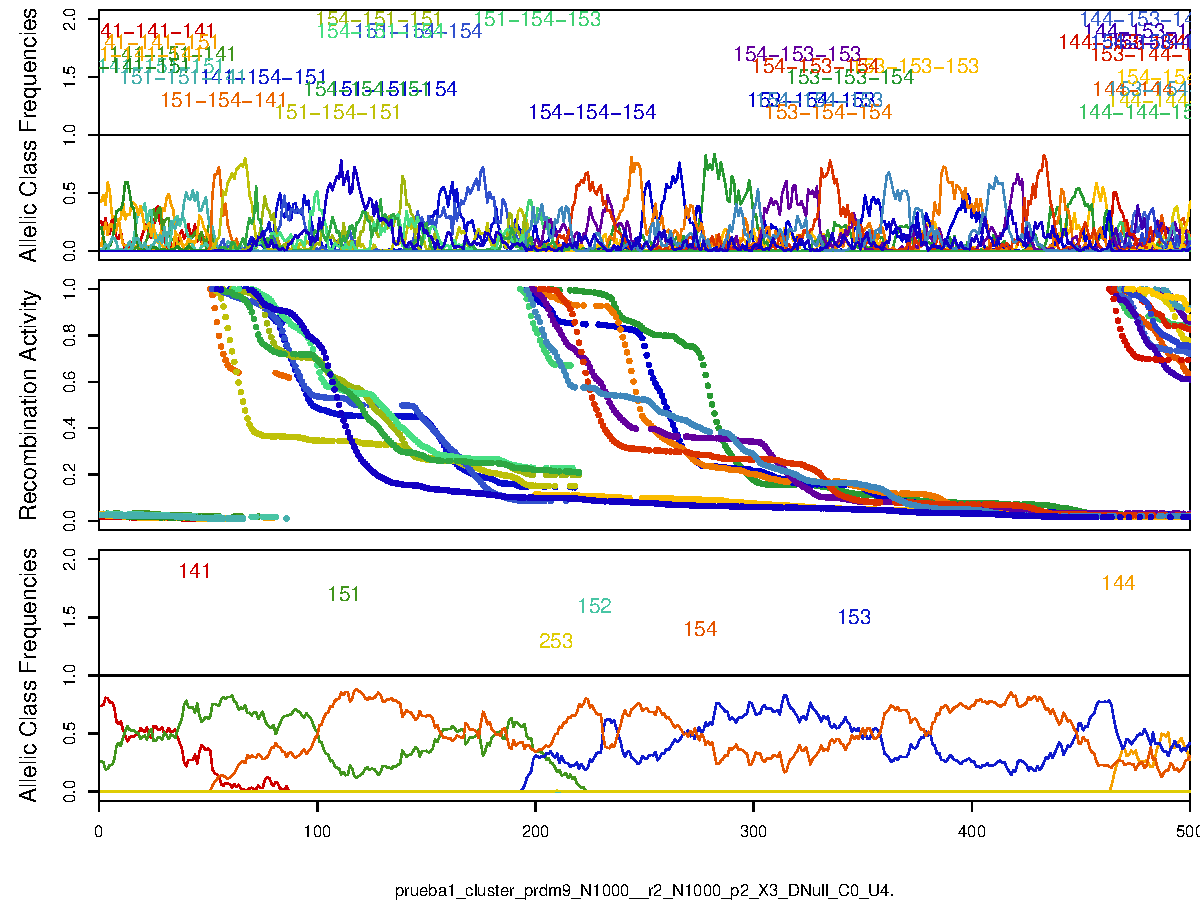
\includegraphics[width=0.95\textwidth] {./Images/prdm9_freqs_labels_C0_U4_b.pdf}
\end{center}

\caption{\small{}}
\label{QuasispeciesExample}
\end{figure}



\section{Origin and success of mutations}

\subsection{Effective mutation rates}
%Let us consider a very simple scenario in which there is no gene conversion between zinc fingers, and that all the mutational input is coming from point mutations. 


Higher interfinger gene conversion rates imply a higher rate of zinc finger homogenization. As such, under a constant point mutation rate and selective pressure, a higher $C$ will imply a smaller ratio of gene conversion events that will actually be a mutation with respect to the total number of gene conversion events (Figure \ref{FigEffMuts}). That is, higher $C$'s will be associated with a higher chance for a gene conversion event to occur between identical zinc fingers, therefore being ``useless''. We observe this phenomenon both for a neutral regime (black simbols in Figure \ref{FigEffMuts}) and under the Red-Queen selective regime. However, the stronger the selective force the higher the proportion of effective gene conversion mutation events. The higher the selection coefficient, the higher the turnover rate, and the higher the chance for individuals carrying new mutations to invade the population, increasing the chance for gene conversion events to be diversifying. In the case of very high mutation rates and low gene conversion rates, differences between neutral and selective regimes is very small. Additionally, lower point mutation rates imply a lower ratio of effective gene conversion mutations. The reason for the latter observation is that higher point mutation generates diversity whereupon gene conversion can act, esentially by transferring ``new'' zinc fingers, generated by point mutations, to the relevant zinc fingers in the array. From this analysis, it is clear that there is a relationship between gene conversion and point mutation rates. 

By increasing gene conversion rate, \textit{ceteris paribus}, there is practically no change in the ratio of effective point mutations relative to the total, except for very high gene conversion rate and point mutation rates, in which we do observe a slight decrease. This makes sense since the homogeneization of zinc fingers does not affect the probability for a new point mutation to generate a new allelic class. Higher selective coefficients increase the ratio of effective point mutations. %This effect might be caused by recurrent mutations, which increase for smaller turnover rates (although I'm not completely certain). 
On the contrary, a higher point mutation rate decreases the ratio of effective point mutations. 

\begin{figure}[htb]
\begin{center}
\leavevmode
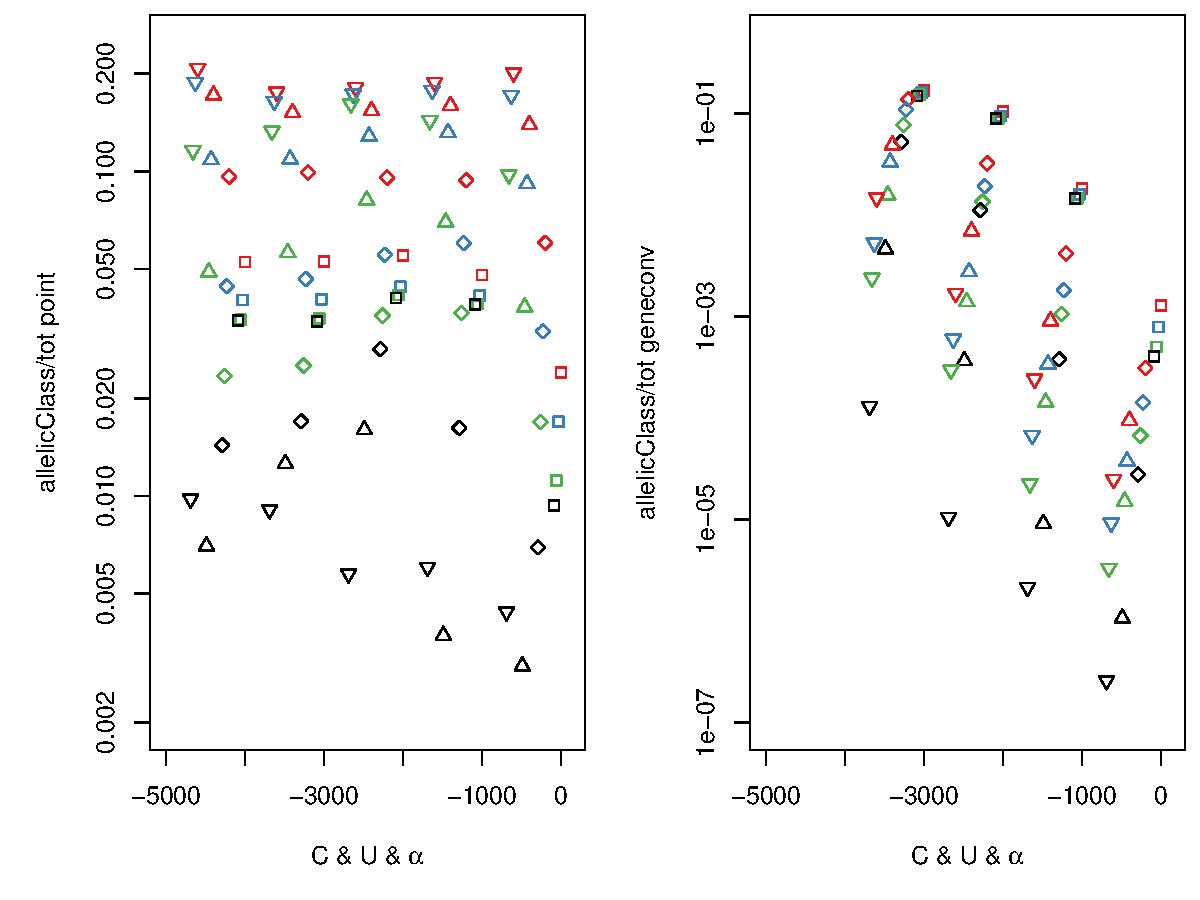
\includegraphics[width=0.95\textwidth] {./Images/Rplot_allelicClassEffVsTot_pointGeneconv.pdf}
\end{center}
\caption{\small{}}
\label{FigEffMuts}
\end{figure}

So, it is clear that there is a link between point mutation and gene conversion that determines the possibility to generate diversifying mutations. A question that we might ask is what is the proportion of new allelic classes generated by point mutation versus those generated by gene conversion mutations. If we ignore the neutral regime, it turns out that the regimes for which the strength of selection (i.e. 4Ns, not to be confused with the selection parameter $\alpha$) is higher are the regimes for which the proportion of new allelic classes generated by gene conversion is highest (see image of gene conversion proportion and 4Ns, red inverted triangles). There are several things of interest regarding these data points: first, the gene conversion effective proportion does not depend on gene conversion rate despite there being four orders of magnitude between different gene conversion rates; second, they correspond to the scenarios of very low point mutation rates; and third, they are the cases for which the efficiency of point mutations is highest (see Figure \ref{FigEffMuts}). 

The fact that both the proportion of effective mutations arising from gene conversion and the fraction of effective point mutations are constant in this scenario of very low mutation rates is in agreement with the mechanism of generation of new allelic classes.
%\begin{enumerate}
% \item A new zinc finger appears in the zinc finger array via point mutation. 
% \item This zinc finger might be born within the binding portion of the array. If it born outside, a gene conversion event might copy this zinc finger to the binding portion of the array.
%  \item Thereafter, gene conversion event can generate many novel allelic classes by copying this zinc finger to other positions within the relevant portion of the array. 
% \item The number of different allelic classes that will contain a particular zinc finger within its binding portion will depend on several parameters and will define the regime in which it is evolving (strong quasi-species vs. weak quasi-species vs. polymorphic vs. sequential).
%\end{enumerate}

%This is a very clear example of the relationship between gene conversion and point mutation rates. In 
For example, in the case of a very low point mutation rate, no matter how high the gene conversion rate, the number of events that will be of use will depend on the availability of segregating zinc fingers, which is dependent on point mutation rate and gene conversion rate. 

For very high gene conversion rates we observe that even the effectivity of point mutations is lower (due mostly to recurrent mutations, most probably). If we look at the proportion of novel allelic classes generated by gene conversion we see that it is extremely low for low gene conversion rates (all new allelic classes are generated by point mutations) and up to 50\% for high gene conversion rates. When comparing this scenario for different values of $\alpha$ we observe that the allelic classes generated by gene conversion are not because of the Red-Queen dynamics since the results for $\alpha=0$ are the same. The only difference between different values of $\alpha$ can be observed for high gene conversion rates. This scenario represents the upper end in point mutation rates, which is up to a point in which gene conversion causes a very small effect. The scenarios in between are the interesting ones, in which there is an interesting equilibrium between gene conversion and point mutation rates. 


%I really do need to check how many of these point mutations generate a new allelic class but not a novel one. 




\subsection{Zinc finger invasions}
There are three possible ways in which a new invading zinc finger can be generated. The first is by having a point mutation in one of the relevant zinc fingers, which will have a high chance to be positively selected. The second is by having a point mutation create a new zinc finger outside the relevant positions and then have gene conversion copy that zinc finger to the relevant positions, within which it can then be selected and rise in frequency. The third possibility is for a new zinc finger to appear outside the relevant positions but in an allele that is rising in frequency in the population, so the novel zinc finger can get to hitchhike and increse its frequency. Here we measuere the proportion of zinc fingers originally generated within the relevant positions. We can see that higher point mutation is the strongest determinant of this proportion and not gene conversion. 

Under no gene conversion we could expect the proportion of zinc fingers born within the relevant positions to be 0.3 (3 out of 10 zinc fingers are relevant). We observe that this is not the case at all, except for high point mutation rates. What does this mean? First, that high gene conversion rates take the system to a neutral regime except when compensated by a high gene conversion rate. Under a neutral regime we could expect the same number of invasions inside than outside of the relevant positions. 

\subsection{Alpha and rho scaling}


\section{Extensions and robustness of the model}

We have explored additional aspects of PRDM9 evolution by extending the model in several directions. Overall, our main model has proven to be robust to extensions and deviations. In particular, we have included duplication and deletion of zinc fingers, we have run simulations under a broad range of population sizes, and we have explored the effects of more realistic gene conversion models. 

\subsection{Duplication and deletion}

\begin{itemize}
\item We introduced the possibility for the zinc finger array to duplicate or delete any one zinc finger at any generation. This introduces variation in the zinc finger array lengths. 
\item Deletion was impeded for alleles with array lengths of 5 zinc fingers, and duplication was impeded for array lengths of 20. 
\item For equal deletion and duplication rates, under the Red-Queen model, zinc finger array length tends to decrease. This implies a selection for shorter zinc finger arrays. The explanation is that generation of novel allelic classes is deletion biased. That is, new allelic classes are generated by a deletion with a higher rate than by a duplication. If, for example, we take an allele whose zinc fingers are all different, a zinc finger duplication will modify its allelic class only if it occurs in a fraction of the binding portion of the array. In particular, if there are Nbind binding zinc fingers, only duplication events at Nbind-1 positions will modify the allelic class, wheareas a deletion of any zinc finger will modify its allelic class. For high gene conversion rates, homogenization of the array diminishes this difference.
\item There could potentially be second order selection on array size if the probability to generate a new allelic class were dependent on the size of the array. For example, it seems plausible that PRDM9 alleles with longer zinc fingers array could contain a higher zinc finger diversity and have a higher probability for a gene conversion event to convert their allelic class. In this scenario, longer array lengths might be indirectly selected because of their larger ``mutational reservoir''. For acceptable gene conversion rates, the deletion bias mentioned above is a much stronger force. However, we do observe second order selection of array length for very high gene conversion rates in which case, deletion bias is minimized due to array homogeneization and very long arrays do contain a larger diversity of zinc fingers and hence a larger mutational reservoir.
\item We did not explore unbalanced duplication and deletion rates. 
\end{itemize}


\subsection{Gene conversion models}
\begin{itemize}
\item Allowing gene conversion to convert zinc fingers incompletely (i.e. having gene conversion tract lenghts that do not begin and/or end at the beginning or end of a zinc finger) makes gene conversion, \textit{a priori}, a mutational force in the sense that it can also generate new zinc fingers, whereas in our basic gene conversion model, new zinc fingers can only arise by point mutation. Basically, it allows for the generation of new zinc fingers by recombination of previously existing ones. 
\item The conclusion of the original model hold. 
\item We do observe an increase in diversity but it is not as high as orginally expected. 
\item There is one observarion regarding selective versus neutral scenarios which was completely unexpected. 
\end{itemize}

\subsection{Population size}
%\begin{itemize}
 
%\end{itemize}




\section{Supplementary material}

\subsection{Master plot}

Behold, the master plot! 
... welcome to 4D abstraction in Figure \ref{RDZs_plot}.

\begin{figure}[htb]
\begin{center}
\leavevmode
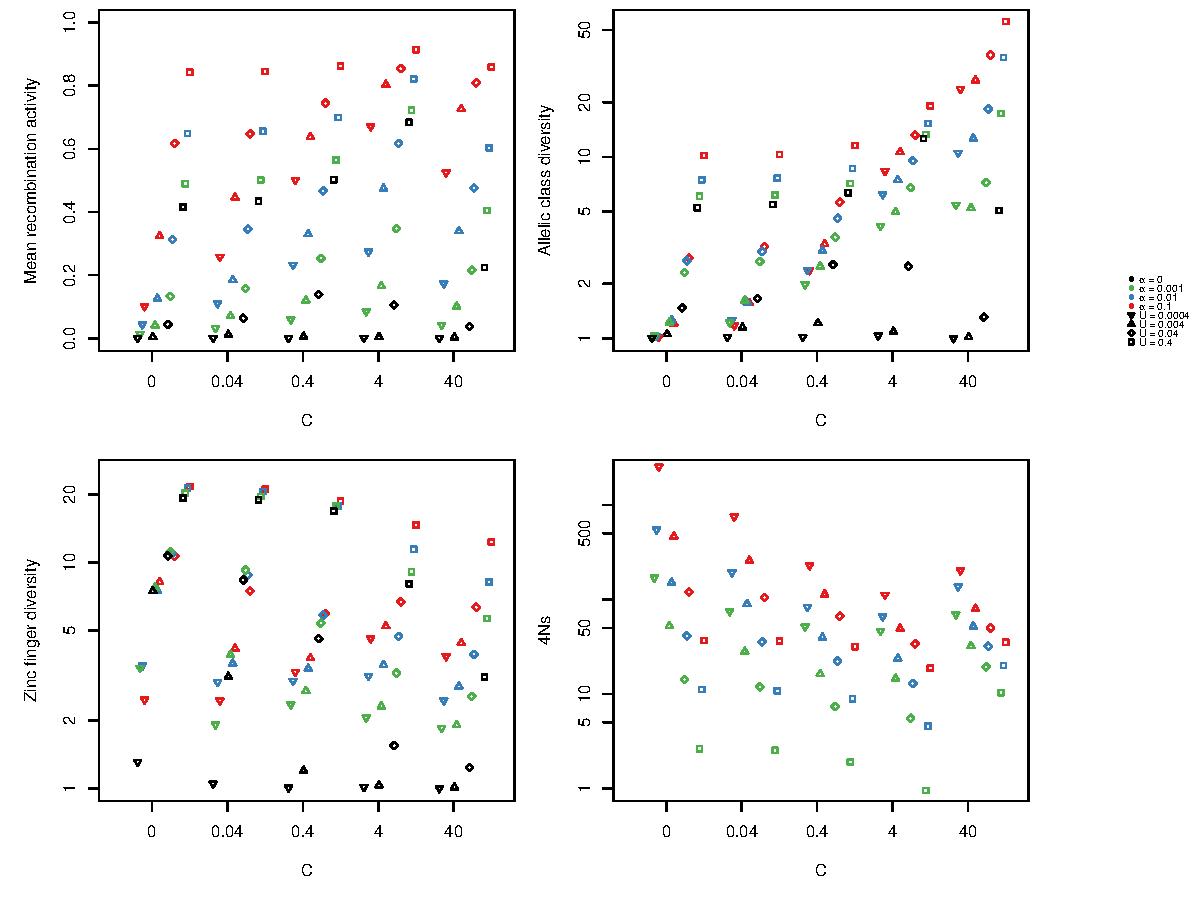
\includegraphics[width=0.95\textwidth] {./Images/prdm9_RDZs_Nulls.pdf}
\end{center}
\caption{\small{}}
\label{RDZs_plot}
\end{figure}

%\bibliography{library}
\bibliography{pzife_biblio}

\end{document}